\documentclass[10pt]{article}
%\usepackage[UTF8]{ctex}

\usepackage[utf8]{inputenc} % allow utf-8 input

\usepackage{amsmath,amscd}
\usepackage{amssymb,array}
\usepackage{amsfonts,latexsym}
\usepackage{graphicx,subfig,wrapfig}
\usepackage{times}
\usepackage{psfrag,epsfig}
\usepackage{verbatim}
\usepackage{tabularx}
\usepackage[pagebackref=true,breaklinks=true,letterpaper=true,colorlinks,bookmarks=false]{hyperref}
\usepackage{cite}
\usepackage{algorithm}
\usepackage{multirow}
\usepackage{caption}
\usepackage{algorithmic}
\usepackage[amsmath,thmmarks]{ntheorem}

% Default fixed font does not support bold face
\DeclareFixedFont{\ttb}{T1}{txtt}{bx}{n}{12} % for bold
\DeclareFixedFont{\ttm}{T1}{txtt}{m}{n}{12}  % for normal

\usepackage{color}
\definecolor{backcolour}{rgb}{0.95,0.95,0.92}
\definecolor{codegreen}{rgb}{0,0.6,0}
\definecolor{deepblue}{rgb}{0,0,0.5}
\definecolor{deepred}{rgb}{0.6,0,0}
\definecolor{deepgreen}{rgb}{0,0.5,0}
\usepackage{listings}

% Python style for highlighting
\newcommand\pythonstyle{\lstset{
		language=Python,
	    backgroundcolor=\color{backcolour},   
		basicstyle=\ttm,
		commentstyle=\color{codegreen},
		morekeywords={self},              % Add keywords here
		keywordstyle=\ttb\color{deepblue},
		emph={MyClass,__init__},          % Custom highlighting
		emphstyle=\ttb\color{deepred},    % Custom highlighting style
		stringstyle=\color{deepgreen},
		breaklines=true,                 
		captionpos=b,                    
		keepspaces=true,                 
		numbers=left,                    
		numbersep=5pt,
		frame=tb,                         % Any extra options here
		showstringspaces=false
}}


% Python environment
\lstnewenvironment{python}[1][]
{
	\pythonstyle
	\lstset{#1}
}
{}

% Python for external files
\newcommand\pythonexternal[2][]{{
		\pythonstyle
		\lstinputlisting[#1]{#2}}}

% Python for inline
\newcommand\pythoninline[1]{{\pythonstyle\lstinline!#1!}}


%\usepackage{hyperref}


\newtheorem{thm}{Theorem}
\newtheorem{mydef}{Definition}

\DeclareMathOperator*{\rank}{rank}
\DeclareMathOperator*{\trace}{trace}
\DeclareMathOperator*{\acos}{acos}
\DeclareMathOperator*{\argmax}{argmax}


\renewcommand{\algorithmicrequire}{ \textbf{Input:}}     
\renewcommand{\algorithmicensure}{ \textbf{Output:}}
\renewcommand{\mathbf}{\boldsymbol}
\newcommand{\mb}{\mathbf}
\newcommand{\matlab}[1]{\texttt{#1}}
\newcommand{\setname}[1]{\textsl{#1}}
\newcommand{\Ce}{\mathbb{C}}
\newcommand{\Ee}{\mathbb{E}}
\newcommand{\Ne}{\mathbb{N}}
\newcommand{\Se}{\mathbb{S}}
\newcommand{\norm}[2]{\left\| #1 \right\|_{#2}}

\newenvironment{mfunction}[1]{
	\noindent
	\tabularx{\linewidth}{>{\ttfamily}rX}
	\hline
	\multicolumn{2}{l}{\textbf{Function \matlab{#1}}}\\
	\hline
}{\\\endtabularx}

\newcommand{\parameters}{\multicolumn{2}{l}{\textbf{Parameters}}\\}

\newcommand{\fdescription}[1]{\multicolumn{2}{p{0.96\linewidth}}{
		
		\textbf{Description}
		
		#1}\\\hline}

\newcommand{\retvalues}{\multicolumn{2}{l}{\textbf{Returned values}}\\}
\def\0{\boldsymbol{0}}
\def\b{\boldsymbol{b}}
\def\bmu{\boldsymbol{\mu}}
\def\e{\boldsymbol{e}}
\def\u{\boldsymbol{u}}
\def\x{\boldsymbol{x}}
\def\v{\boldsymbol{v}}
\def\w{\boldsymbol{w}}
\def\N{\boldsymbol{N}}
\def\X{\boldsymbol{X}}
\def\Y{\boldsymbol{Y}}
\def\A{\boldsymbol{A}}
\def\B{\boldsymbol{B}}
\def\y{\boldsymbol{y}}
\def\cX{\mathcal{X}}
\def\transpose{\top} % Vector and Matrix Transpose

%\long\def\answer#1{{\bf ANSWER:} #1}
\long\def\answer#1{}
\newcommand{\myhat}{\widehat}
\long\def\comment#1{}
\newcommand{\eg}{{e.g.,~}}
\newcommand{\ea}{{et al.~}}
\newcommand{\ie}{{i.e.,~}}

\newcommand{\db}{{\boldsymbol{d}}}
\renewcommand{\Re}{{\mathbb{R}}}
\newcommand{\Pe}{{\mathbb{P}}}

%\hyphenation{MATLAB}

\usepackage[margin=1in]{geometry}

\begin{document}
	
\title{	Machine Learning, 2021 Spring\\Homework 3}
\date{Due on 23:59 APR 7, 2021}
\maketitle

%%%%%--------------------

\section{Training Logistic Regression Models via Scikitlearn}
\subsection{Dependencies:}
This homework requires a \textbf{python} implementation. Followings are the packages this work may depend on:
\begin{itemize}
	\item Scikitlearn: \url{https://scikit-learn.org/stable/install.html},
	\item Numpy: \url{https://numpy.org/install/},
	\item Matplotlib: \url{https://matplotlib.org/stable/users/installing.html}.
\end{itemize}
We strongly recommend that you use Anaconda to install them.

\subsection{Your tasks:}
We provide three data sets from Scikitlearn: 
\begin{enumerate}
	\item $\mathcal{D}_1$: an almost linearly separable data set,
	\item $\mathcal{D}_2$: a ``moon''-like data set,
	\item $\mathcal{D}_3$: a ``circle''-like data set. 
\end{enumerate}
Please train logistic regression classifiers on these three data sets. Note that you \textbf{do not} need to write a logistic regression model by yourself, just use the one provided in Scikitlearn.
We left the requirement details for each data set in the following. For your convenience, we also provide a jupyter notebook for the code (named `hw3.ipynb'). You can find the data sets generation part in file \emph{data.py} as well.

\subsubsection*{Task I:}\label{s.T1}

After executing the data generation code for Task I, you can get a scatter plotting of the data points as shown in \ref{fig.fig1}.
\begin{figure}[h!]
	\centering
	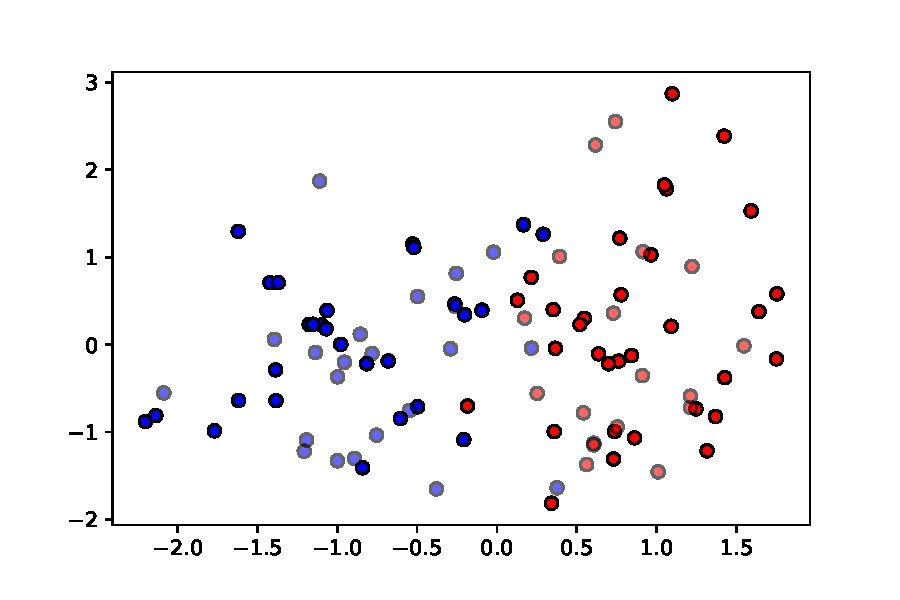
\includegraphics[width=0.7\linewidth]{fig1}
	\caption{The linearly separable data set.}
	\label{fig.fig1}
\end{figure}

{\color{red}Problem 1:} It is your turn to use the logistic regression model (module \emph{linear\_model.LogisticRegression} in Scikitlearn) for training a linear classifier on $\mathcal{D}_1$. \textbf{You need to:} {\color{red}[3pts]}
\begin{enumerate}
	\item[(i)] provide the specific values of parameters you choose, e.g., \emph{tol} (tolerance), \emph{max\_iter};
	\item[(ii)] report the score of your classifier (the mean accuracy on the given test data and labels);
	\item[(iii)] plot your decision boundary (actually a line in this 2-dimension case). \\
	(\textbf{Hint:} you can refer to the example code provided in ``Task II'' for the details of plotting.)
	
\end{enumerate}


\subsubsection{Task II:}
After executing the data generation code for Task II, you can  get the scatter plotting of the data points as shown in \ref{fig.fig2}.

\begin{figure}[H]
	\centering
	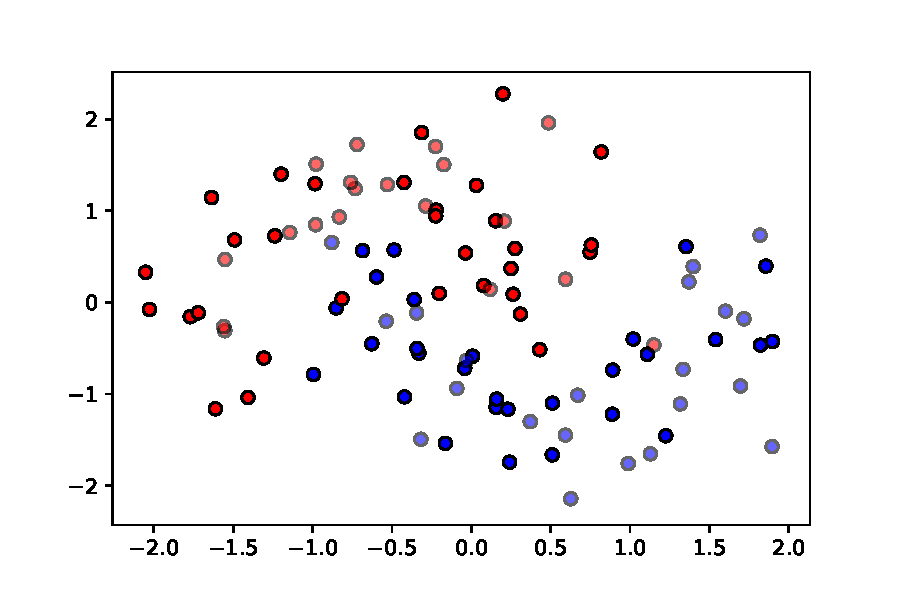
\includegraphics[width=0.7\linewidth]{fig2}
	\caption{The ``moon''-like data set.}
	\label{fig.fig2}
\end{figure}

{\color{red}Problem 2:} It is your turn to use the logistic regression model (module \emph{linear\_model.LogisticRegression} in Scikitlearn) for training a linear classifier on $\mathcal{D}_2$. \textbf{You need to:} {\color{red}[3pts]}
\begin{enumerate}
	\item[(i)] provide the specific values of parameters you choose;
	\item[(ii)] report the score of your classifier (the mean accuracy on the given test data and labels);
	\item[(iii)] plot your decision boundary (actually a line in this 2-dimension case).  
\end{enumerate}

Let us think a little bit further of this task.
While finishing the training of this task, you may not completely satisfy with the classifier you have got, since you can not fit a linearly non-separable data set well with a linear classifier. Unfortunately, the logistic regression model is essentially a linear model. However, we are not at a loss what to do. 

Often it’s useful to add complexity to the model by considering nonlinear features of the input data. A simple and common method to use is polynomial features, which can get features’ high-order and interaction terms. For example, if we perform a polynomial transformation with degree$=2$ on features $(x_1, x_2)$, they will be transformed to $(1, x_1, x_2, x_1^2, x_1 x_2, x_2^2)$. Then, training a linear model on the transformed data set will lead to a polynomial model of the original data set. We will not go further for the theoretical analysis, instead providing the implementation and the associated results, which is called the kernel method.
 
\begin{python}
'''Define polynomial regression, the value of degree can adjust
the characteristics of polynomial'''
poly_reg = PolynomialFeatures(degree=3) 
# Feature processing (get the sample data corresponding to the corresponding feature of the polynomial)
X_poly = poly_reg.fit_transform(X)

# Training model
model = linear_model.LogisticRegression()
model.fit(X_poly, y)

'''The returned estimates for all classes are ordered by the label of classes.'''
z = model.predict_proba(poly_reg.fit_transform(np.c_[xx.ravel(), yy.ravel()]))[:, 1]
# '''Predict class labels for samples in X.'''
# z = model.predict(poly_reg.fit_transform(np.c_[xx.ravel(), yy.ravel()]))

z = z.reshape(xx.shape)
score = model.score(X_poly, y)

# Plot the contour of the classifier
plt.contourf(xx, yy, z, cmap=cm, alpha=.8)
# Plot the training points
plt.scatter(X_train[:, 0], X_train[:, 1], c=y_train, 
cmap=cm_bright, edgecolors='k')
# Plot the testing points
plt.scatter(X_test[:, 0], X_test[:, 1], c=y_test, cmap=cm_bright,
edgecolors='k', alpha=0.6)

name = 'Logistic Regression'
plt.title(name)
plt.text(xx.max() - .3, yy.min() + .3, ('%.3f' % score),
size=15, horizontalalignment='right')
fig2p = plt.gcf()
plt.show()
\end{python}

Then we get the classifier shown in Figure \ref{fig.fig2p}. (We only focus on the classification performance and do not take the generalization of the model into account of this task.)
\begin{figure}[h!]
	\centering
	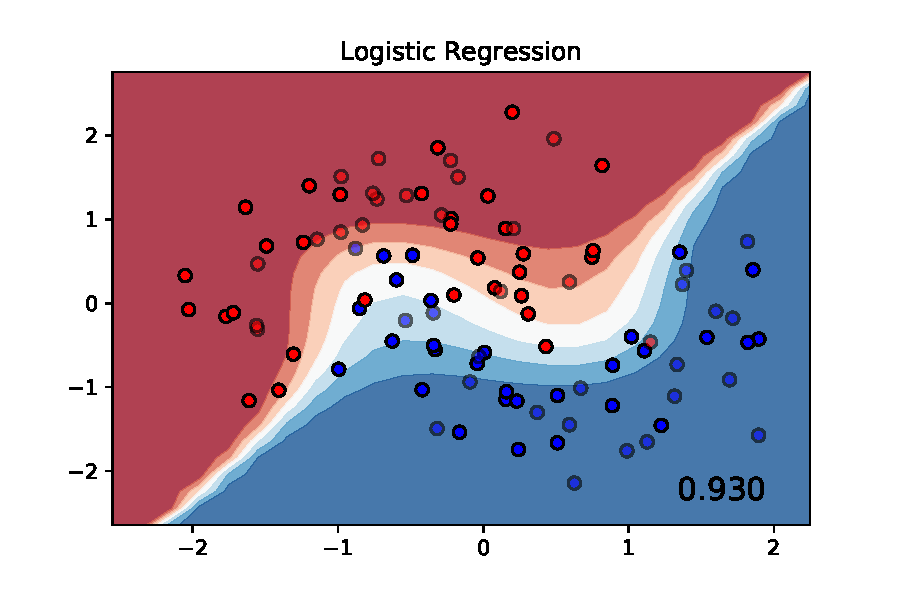
\includegraphics[width=0.7\linewidth]{fig2pl}
	\caption{Polynomial transformed classifier.}
	\label{fig.fig2p}
\end{figure}

\newpage
\subsubsection{Task III:}
After executing the data generation code for Task III, you can get the scatter plotting of the data points as shown in \ref{fig.fig2}.

\begin{figure}[h!]
	\centering
	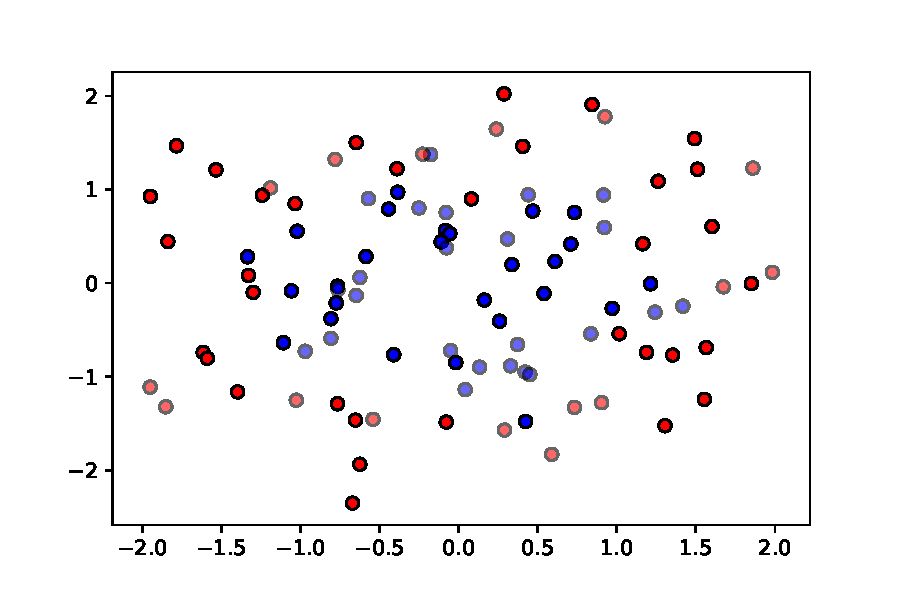
\includegraphics[width=0.7\linewidth]{fig3}
	\caption{The ``circle''-like data set.}
	\label{fig.fig3}
\end{figure}

{\color{red}Problem 3:} It is your turn to use the logistic regression model (module \emph{linear\_model.LogisticRegression} in Scikitlearn) for training a linear classifier on $\mathcal{D}_3$. \textbf{You need to:} {\color{red}[2pts]}
\begin{enumerate}
	\item[(i)] provide the specific values of parameters you choose;
	\item[(ii)] report the score of your classifier (the mean accuracy on the given test data and labels);
	\item[(iii)] plot your decision boundary (actually a line in this 2-dimension case).  
\end{enumerate}
\textbf{Extra task:} perform a polynomial transformation on $\mathcal{D}_3$ and re-train a logistic regression classifier on the transformed data set. \textbf{You need to:} {\color{red}[2pts]}
\begin{enumerate}
	\item[(i)] provide the specific values of parameters you choose;
	\item[(ii)] report the score of your classifier (the mean accuracy on the given test data and labels);
	\item[(iii)] plot your decision boundary (actually a line in this 2-dimension case).  
\end{enumerate}


\end{document} 